\documentclass[convert={density=900,size=1080x800,outext=.png}]{standalone}
\usepackage{tikz}
\usetikzlibrary{calc, positioning}
\usetikzlibrary{arrows.meta}
\usetikzlibrary{matrix}
\usetikzlibrary{shadows}
\usepgflibrary{shapes.misc}
\usepgflibrary{{shapes.geometric}}
\usetikzlibrary{arrows,positioning,shapes}

\pgfdeclarelayer{shadow} 
\pgfsetlayers{shadow,main}
\def\shadowradius{3pt}


\def\lw{2mm}        % Arrow line width
\def\mw{2cm}        % Minimum width of component
\def\mh{1.75cm}     % Minimum height of component
\def\trianglecoordinate{2mm}    % Starting coordinate clock input triangle of components

\newcommand\drawshadowbis[1]{
    \begin{pgfonlayer}{shadow}
        \fill[inner color=black,outer color=white] ($(#1.south west)$) circle (\shadowradius);
        \fill[inner color=black ,outer color=white] ($(#1.north west)$) circle (\shadowradius);
        \fill[inner color=black ,outer color=white] ($(#1.south east)$) circle (\shadowradius);
        \fill[inner color=black,outer color=white] ($(#1.north east)$) circle (\shadowradius);
        \fill[ top color=black, bottom color=white] ($(#1.south west)+((0,-\shadowradius)$) rectangle ($(#1.south east)$);
        \fill[left color=black,right color=white] ($(#1.south east)$) rectangle ($(#1.north east)+((\shadowradius,0)$);
        \fill[bottom color=black,top color=white] ($(#1.north west)$) rectangle ($(#1.north east)+((0,\shadowradius)$);
        \fill[right color=black,left color=white] ($(#1.south west)$) rectangle ($(#1.north west)+(-\shadowradius,0)$);
    \end{pgfonlayer}
    }

\tikzset{
    border/.style = { 
        draw, rectangle, minimum width=2cm, minimum height=1.5cm, thick
    },
    pics/Component/.style n args = {2}{
        code = {
            \node [border, align=center](-edge){#1};
            \draw[thick] ([xshift=\trianglecoordinate] -edge.south) -- ([yshift=\trianglecoordinate] -edge.south);
            \draw[thick] ([xshift=-\trianglecoordinate] -edge.south) -- ([yshift=\trianglecoordinate] -edge.south);
            \draw[thick] (-edge.south) |- ++(-3mm, -4mm) node[xshift=-2mm, yshift=-1mm] {#2}; 
    }}
    }


\begin{document}
    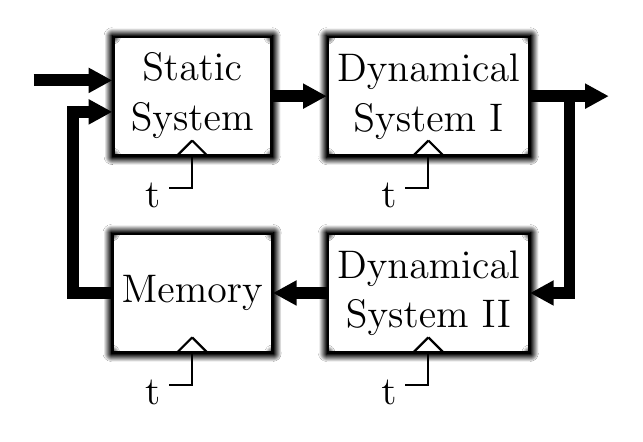
\begin{tikzpicture}[every node/.style={font=\Large}]
        % Place the blocks 
        \draw pic (b1) {Component={Static\\System}{t}};
        \draw(3, 0) pic (b2) {Component={Dynamical\\System I}{t}};
        \draw(3, -2.5) pic (b3) {Component={Dynamical\\System II}{t}};
        \draw(0, -2.5) pic (b4) {Component={Memory}{t}};
        % Glow the blocks
        \drawshadowbis{b1-edge};
        \drawshadowbis{b2-edge};
        \drawshadowbis{b3-edge};
        \drawshadowbis{b4-edge};
        \begin{scope}[line width=1.5mm, >={Triangle[width=3mm,length=3mm]}]
            \draw[->] ([yshift=2mm, xshift=-1cm] b1-edge.west) -- ([yshift=2mm] b1-edge.west);
            \draw[->] (b1-edge.east) -- (b2-edge.west);
            \draw (b2-edge.east) -- ++(0.5cm, 0cm) coordinate (a);
            \draw[->] (a) -- ++(0.5cm, 0cm);
            \draw[->] (a) |- (b3-edge.east);
            \draw[<-] ([yshift=-2mm] b1-edge.west) -- ++(-0.5cm, 0cm) coordinate (b);
            \draw[-] ([yshift=0.75mm] b) |- (b4-edge.west);
            \draw[->] (b3-edge.west) |- (b4-edge.east);
        \end{scope}
    \end{tikzpicture}
\end{document}
